\section{}
\[
H(s)=\frac{s^2-100}{s+1}=\frac{(s-10)(s+10)}{s+1}\,.
\]
\subsection{Bode-Diagramm}
\begin{center}
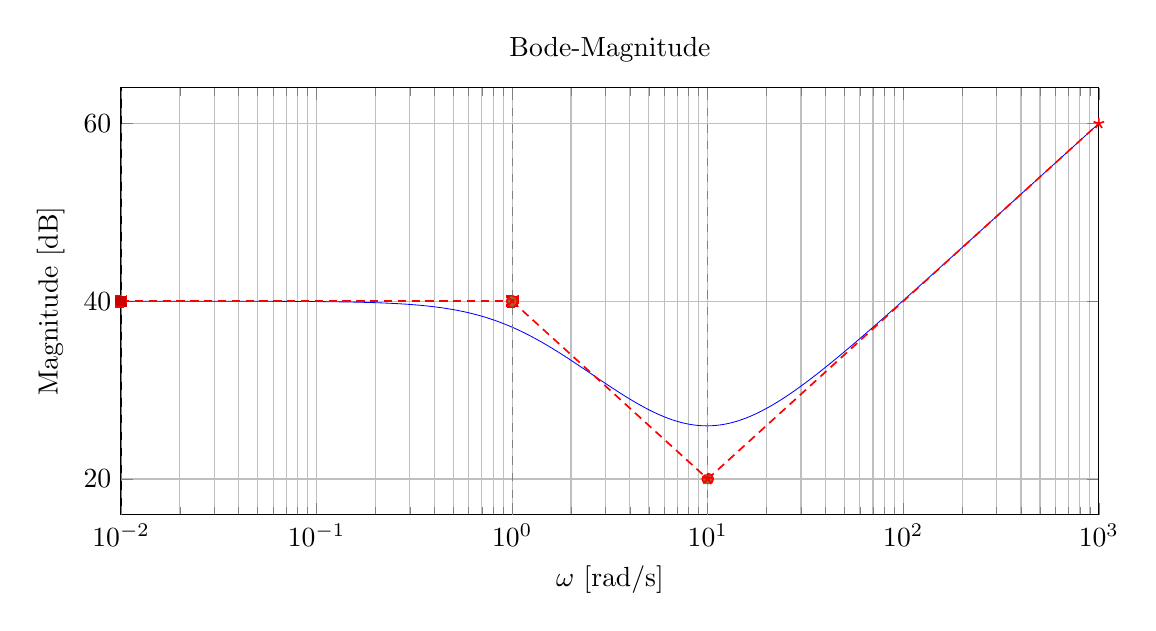
\begin{tikzpicture}
\begin{semilogxaxis}[
  width=14cm,height=7cm,
  xmin=1e-2,xmax=1e3,
  xlabel={$\omega$ [rad/s]},
  ylabel={Magnitude [dB]},
  grid=both,
  ytick distance=20,
  title={Bode-Magnitude}
]
\addplot[
  domain=1e-2:1e3,
  samples=600,
  mark=none,
  line width=0.3pt,
  blue
] {40*ln(sqrt(100 + x^2))/ln(10) - 20*ln(sqrt(1 + x^2))/ln(10)};
\addplot+[domain=1e-2:1,samples=2,dashed,dash pattern=on 3pt off 2pt,line width=0.6pt,red] {40};
\addplot+[domain=1:1e1,samples=2,dashed,dash pattern=on 3pt off 2pt,line width=0.6pt,red] {40 - 20*ln(x)/ln(10)};
\addplot+[domain=1e1:1e3,samples=2,dashed,dash pattern=on 3pt off 2pt,line width=0.6pt,red] {20 + 20*ln(x/10)/ln(10)};
\draw[gray,dashed] (rel axis cs:0,0) -- (rel axis cs:0,1);
\draw[gray,dashed] (axis cs:1,\pgfkeysvalueof{/pgfplots/ymin}) -- (axis cs:1,\pgfkeysvalueof{/pgfplots/ymax});
\draw[gray,dashed] (axis cs:10,\pgfkeysvalueof{/pgfplots/ymin}) -- (axis cs:10,\pgfkeysvalueof{/pgfplots/ymax});
\node[gray,anchor=south east] at (axis cs:1,\pgfkeysvalueof{/pgfplots/ymax}) {\scriptsize Pol $\omega_p=1$};
\node[gray,anchor=south east] at (axis cs:10,\pgfkeysvalueof{/pgfplots/ymax}) {\scriptsize Nullstellen $\omega_z=10$ (LHP \& RHP)};
\end{semilogxaxis}
\end{tikzpicture}
\vspace{6mm}
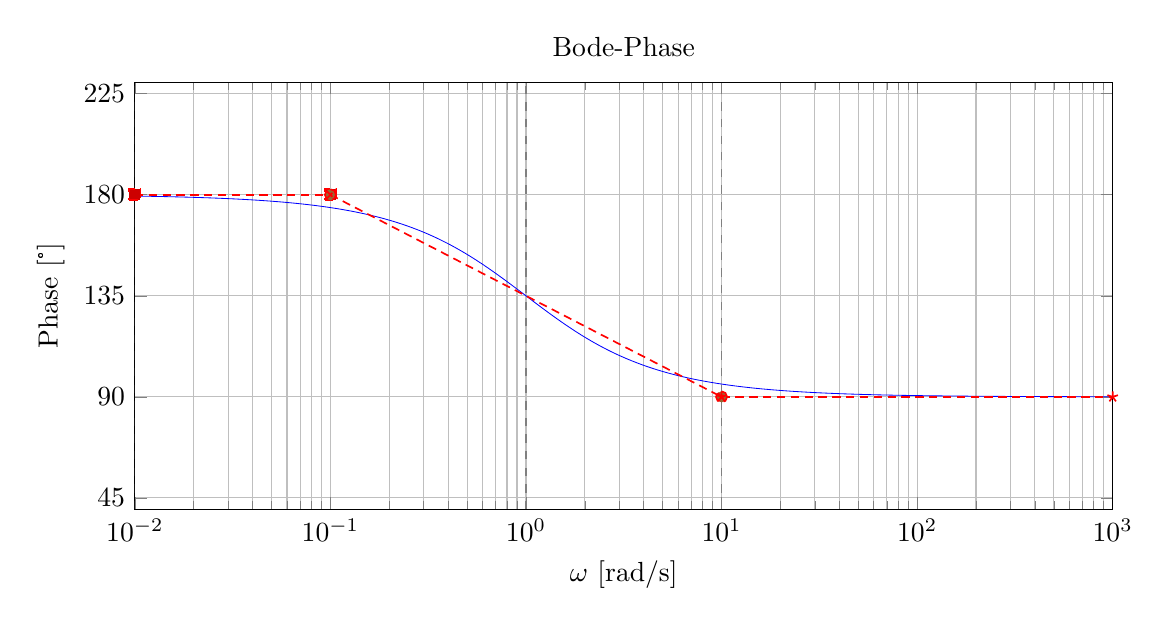
\begin{tikzpicture}
\begin{semilogxaxis}[
  width=14cm,height=7cm,
  xmin=1e-2,xmax=1e3,
  ytick distance=45,
  ymin=40,ymax=230,
  xlabel={$\omega$ [rad/s]},
  ylabel={Phase [°]},
  grid=both,
  title={Bode-Phase}
]
\addplot[
  domain=1e-2:1e3,
  samples=600,
  mark=none,
  line width=0.3pt,
  blue
] {180 - atan(x)};
\addplot+[domain=1e-2:1e-1,samples=2,dashed,dash pattern=on 3pt off 2pt,line width=0.6pt,red] {180};
\addplot+[domain=1e-1:1e1,samples=2,dashed,dash pattern=on 3pt off 2pt,line width=0.6pt,red] {135 - 45*ln(x)/ln(10)};
\addplot+[domain=1e1:1e3,samples=2,dashed,dash pattern=on 3pt off 2pt,line width=0.6pt,red] {90};
\draw[gray,dashed] (rel axis cs:0,0) -- (rel axis cs:0,1);
\draw[gray,dashed] (axis cs:1,\pgfkeysvalueof{/pgfplots/ymin}) -- (axis cs:1,\pgfkeysvalueof{/pgfplots/ymax});
\draw[gray,dashed] (axis cs:10,\pgfkeysvalueof{/pgfplots/ymin}) -- (axis cs:10,\pgfkeysvalueof{/pgfplots/ymax});
\node[gray,anchor=south east] at (axis cs:1,\pgfkeysvalueof{/pgfplots/ymax}) {\scriptsize Pol $\omega_p=1$};
\node[gray,anchor=south east] at (axis cs:10,\pgfkeysvalueof{/pgfplots/ymax}) {\scriptsize Nullstellen $\omega_z=10$ (LHP \& RHP)};
\end{semilogxaxis}
\end{tikzpicture}
\end{center}
\newpage
\subsection{Erklärung}
\vspace{5mm}
\begin{description}[leftmargin=1.2em,labelsep=.6em,font=\bfseries]
\item[Schritt 1] Struktur: $H(s)=\dfrac{(s-10)(s+10)}{s+1}$. Für $\omega\ll1$ ist $|H(\j\omega)|\approx\dfrac{100}{1}=100\Rightarrow 40\,\mathrm{dB}$ ohne Startsteigung. $H(0) = -100 = 100 e^{+j180^\circ}$ $\Rightarrow$ konstante Phasenlage $+180^\circ$.
\item[Schritt 2] Pol bei $\omega_p=1\,\mathrm{rad/s}$: ab $\omega=1$ Steigungswechsel um $-20\,\mathrm{dB/dec}$; am Eckpunkt exakte Dämpfung $-10\log_{10}2\approx-3\,\mathrm{dB}$ gegenüber der linken Geraden. Phasenabnahme des Pols um $90^\circ$ über $\omega\in[0.1,10]$; Geradennäherung $135^\circ-45^\circ\log_{10}\omega$ (von $180^\circ$ auf $90^\circ$).
\item[Schritt 3] Nullstellen bei $\omega_z=10\,\mathrm{rad/s}$ (eine LHP, eine RHP): Magnitudenbeitrag von zwei Nullstellen $\Rightarrow$ zusätzliche $+40\,\mathrm{dB/dec}$ ab $\omega=10$; Netto-Gesamtslope wird $+20\,\mathrm{dB/dec}$ für $\omega\gg10$. Am Eckpunkt $\omega=10$ liegt $|H(\j10)|_{\mathrm{dB}}\approx20+6=26.0\,\mathrm{dB}$. Die Phasenänderungen der LHP- und RHP-Nullstelle heben sich gegenseitig auf; Netto entsteht an $\omega=10$ keine zusätzliche Phasenänderung (die konstanten $+180^\circ$ sind bereits berücksichtigt).
\end{description}

\vspace{0.5cm}
\medskip
\noindent\textbf{Stückweise Näherung}
\[
|H(\j\omega)|_{\mathrm{dB}}\approx
\begin{cases}
40,& \omega\ll1,\\[4pt]
40-10\log_{10}2,& \omega=1,\\[4pt]
40-20\log_{10}\omega,& 1\ll\omega\ll10,\\[4pt]
20+20\log_{10}(\omega/10),& \omega\gg10,
\end{cases}
\qquad
\]
\newpage